\documentclass{article}

\usepackage{graphicx}
\usepackage[utf8]{inputenc}
\usepackage[a4paper, top=4cm, bottom=4cm, left=4cm, right=4cm]{geometry}

\title{
    \textbf{\textit{SafeStreet}} \\
    \textbf{RASD document}}

\date{Academic year: 2019 - 2020}
\author{
    Dario Miceli Pranio \\
    Pierriccardo Olivieri
}

\begin{document}
\pagenumbering{gobble}

\maketitle

%%%%%%%%%% LOGO POLIMI %%%%%%%%%%
\begin{figure}[h!]
    \centering
    
\includegraphics[scale=0.5]{img/logo.png}
\end{figure}

\newpage
\pagenumbering{arabic}
\tableofcontents

\newpage
%%%%%%%%%% CHAPTER 1 %%%%%%%%%%
\section{Introduction}
This is the RASD document for \textit{SafeStreet}, 
it provides a general view about key aspects of the project. The purpose of this document is to formalize a description
of the system's requirements both functional and non-funcional. In the following pages will be covered goals of the 
application with respect to phenomena. This document is addressed to developers as a guideline to implement the requirements
that follows.  

\subsection{Purpose}
SafeStreets is a service that aims to provide users with the possibility to notify authorities when traffic 
violations occur, and in particular parking violations. The application's goal is achieved by allowing users 
to share photo, position, date, time and type of violation and by enabling \textit{Authorities} to request them.
\\
\\
Safestreets requires the users to create an account to access its services, the functionalities unlocked after 
registration depend on the type of account created.
\\
If a user creates an account as \textit{Citizen}, he/she must provide information about ID card on order to prove 
that he/she is a real person. Furthermore, he must provide an email with which he will be uniquely identified 
and a password. Once the account has been activated, user can finally start to report parking violation. 
The users can also see a summary of the streets with the highest frequency of violations.
\\
\\
On the other hand, an officer will create an account as \textit{Authority} and he will need to provide his name, surname, 
work's Matricola, a password and as for \textit{Citizen}, will be uniquely identified by an email. Once the Matricola 
has been verified and the account has been activated, the officer can retrieve the potential parking violations 
sent by \textit{Citizen} that have not been taken into account yet by other officers, analyze them and, if it is the 
right case, generate traffic tickets. \textit{Authorities} can also see a summary of the vehicles' license plate that 
commit the most violations.
\\
\\
From this brief description of the functionalities we may extract the following goals for SafeStreets:
\begin{itemize}
    \item \textbf{[G1]}: Allow users to be identified as a \textit{Citizen} or as \textit{Authority};
    \item \textbf{[G2]}: Allow \textit{Citizens} to report parking violations;
    \item \textbf{[G3]}: \textit{Citizen} has to be able to input information about the violation that he has reported;
    \item \textbf{[G4]}: Must provide a visualization of the areas with high frequency of violations;
    \item \textbf{[G5]}: \textit{Authority} can retrieve vehicles that commit the most violations; 

\end{itemize}
Safestreets offers also some advanced functions in addition to the basic version.
\begin{itemize}
    \item \textbf{[G6]}: Must ensure the chain of custody of the information sent by \textit{Citizens};
    \item \textbf{[G7]}: \textit{Authority} can retrieve traffic violations' data inserted by \textit{Citizens};
    \item \textbf{[G8]}: Build statistics with the information about issued tickets;
\end{itemize}

\subsection{Scope}
Here we will describe all the relevant phenomena that may occur. 

\subsubsection{World Phenomena}
Those are the events that may occur in the real word and are not affected by the Machine.
\\We identify:
\begin{itemize}
    \item \textit{Citizen} sees a parking violation and wants to report it;
    \item \textit{Authorities} want to know about some violations that have been occurred;
    \item A \textit{parking violation} occurs; 
\end{itemize} 

\subsubsection{Shared Phenomena}
Shared phenomena are the events based on the link beetween World Phenomena and Machine Phenomena.
We can distinguish them in two types:
\\
Controlled by the world observed by the machine:
\begin{itemize}
    \item A Citizen take a photo of a violation;
    \item Users can enter data for registration/login;
    \item Users can request data;
\end{itemize}
Controlled by the machine observed by the world:
\begin{itemize}
    \item track position of the violation;
    \item mark areas with an high rate of violations;
    \item System can fullfill data requests;
\end{itemize}

\subsubsection{Machine Phenomena}
The Machine Phenomena are the events that occur inside the machine and are not affected by the real world.
\\We identify:
\begin{itemize}
    \item storing permanently collected data;
    \item encryption of sensitive data;
    \item retrieving data for a request; 
\end{itemize} 

\subsection{Definitions, acronyms, abbreviations}

\subsubsection{Definitions}
\begin{itemize}
    \item user: can be either citizen or authorities
\end{itemize}
traffic violation: generic violation that can occur in a street
parking violation: a violation caused by a bad parking
violation: general violation, identity both traffic or parking violation
unsafe areas: areas with an high rate of violations

\subsubsection{Acronyms}
Table with all acronyms used in document.
\begin{center}
\begin{tabular}{ | l | l |}
    \hline
    ACRONYM & COMPLETE NAME \\
    \hline
    RASD & Requirements Analysis and Specification Document \\
    \hline
    GPS & global positioning systems \\
    \hline
    ID & Identity document \\
    \hline
    S2B & Software to be \\
    \hline
    GDPR & General Data Protection Regulation \\
    \hline 
\end{tabular}
\end{center}

\subsubsection{Abbreviations}

\subsection{Revision History}

\subsection{Reference documents}

\subsection{Document Structure}
\begin{itemize}
    \item \textbf{Chapter 2:}
    \item \textbf{Chapter 3:}
    \item \textbf{Chapter 4:}  
\end{itemize}
%%%%%%%%%% !CHAPTER 1 %%%%%%%%%%

%%%%%%%%%% CHAPTER 2 %%%%%%%%%%
\section{Overall Description}

\subsection{Product perspective}
This section aims to explain in more detail the World, Machine and Shared Phenomena described in the 
previous Chapter. 
\subsubsection{World Phenomena}
\begin{itemize}
    \item \textbf{Citizen sees a parking violation and wants to report it:}
    While the Citizen is quietly walking, he sees a parking violations like a double parking or a car
    parked in the middle of bike lane so he logs in, takes a picture, inserts the type of violations
    and sends it to the \textit{System}.  
    \item \textbf{Authorities want to know abount some violations that have been occurred:}
    An Authority logs in and retrieves all the violations that have been send by the Citizen 
    \item \textbf{Parking violations occurrs:}
    Someone in the city decides to not follow parking rules and does not park his car in a proper way   
\end{itemize}
\subsubsection{Machine Phenomena}
\begin{itemize}
    
\item \textbf{Storing permanently collected data:}
The system needs to store, in a secure way, all the data submitted.
In order to achive this purpose and guarantee the best service
the system needs to use a DBMS.

\item \textbf{Encryption of sensitive data:}
Personal user's data and all the data relative to the violations
that can only be seen by authorities need to be encrypted in order
to proctect it from non-allowed third parties. 

\item \textbf{Retrieving data for a request:}
System have to fullfill the data request from the users. Data 
requests can be of two types, a Citizen request who want to see
statistics of a certain city area or data request by Authorities
who want to receive the violation reports collected by SafeStreet
\end{itemize}

\subsubsection{Shared Phenomena}
Controlled by the World observed by the Machine
\begin{itemize}
    \item \textbf{A Citizen take a photo of a violation:}
    Situation in which a Citizen spots a generic violation and wants
    to report it through the application. Using the phone camera he
    can take the photo of the violation.

    \item \textbf{User can enter data for registration/login:}
    A user decide to use the application and provides his personal 
    in order to register if it's the first time he use the app, or to
    identify himself.

    \item \textbf{Users can request data:}
    In this phenomena we make a distinction between Citizen and Authorities.
    A Citizen or may want to see violation statistics 
    of a certain area, or in the case of Authorities they can, request
    violation statistics and additional informations 
\end{itemize}

Controlled by the Machine observed by the World
\begin{itemize}
    \item\textbf{Track position of the violation}
    The \textit{System} can retrieve the position where the violation occurred by fetching it from GPS service
    \item\textbf{Mark areas with an high rate of violations}
    Once lots of violations occured, the \textit{System} mines the information that it has in order to highlight the areas with the highest frequency of violations
    \item\textbf{System can fullfill data requests}
    After processing a request, the \textit{System} will show to the user the result of the DBMS query in a proper way

\end{itemize}

\subsubsection{Class Diagram} 

\begin{figure}[h!]
    \centering
    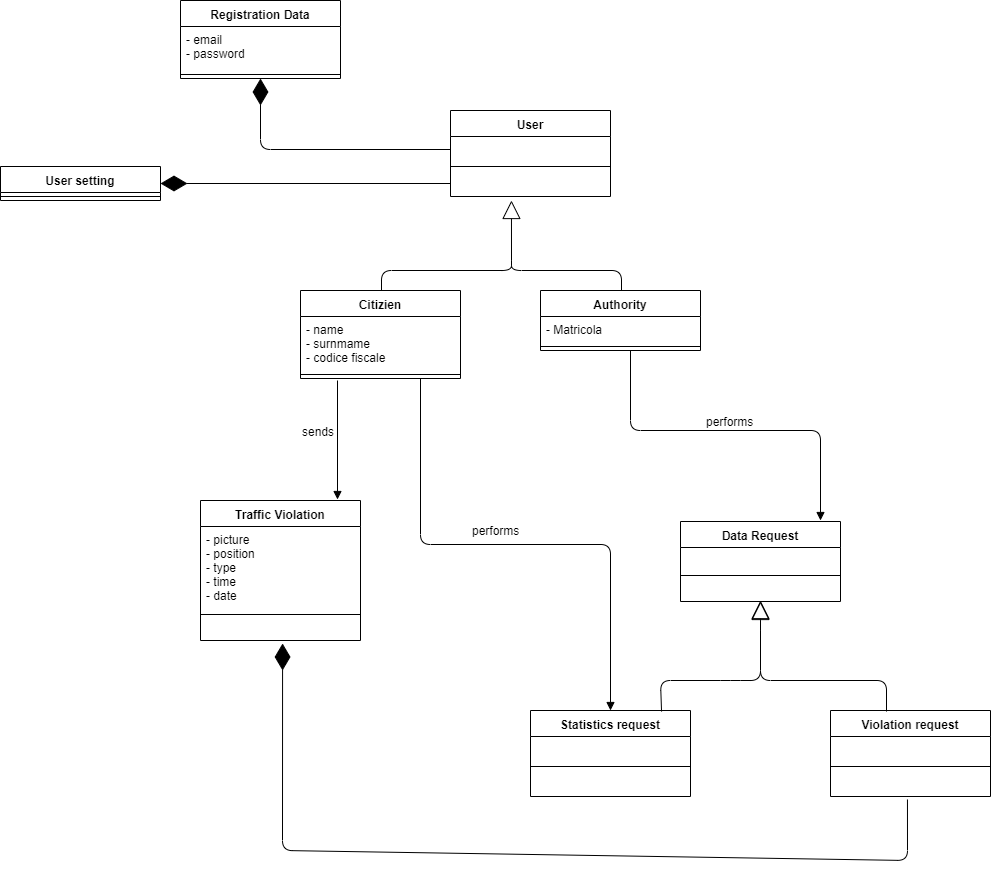
\includegraphics[scale=0.3]{img/Class_Diagram.png}
    \caption{Safestreets' Class diagram}
\end{figure}
\clearpage
\subsubsection{State Chart} 

\begin{figure}[h!]
    \centering
    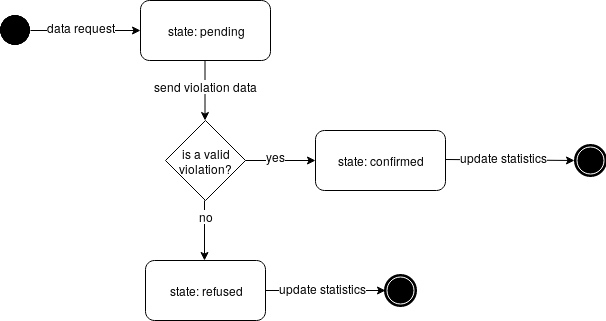
\includegraphics[scale=0.5]{img/authority_request.png}
    \caption{Authority request state chart}
\end{figure}

\begin{figure}[h!]
    \centering
    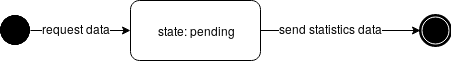
\includegraphics[scale=0.5]{img/citizen_request.png}
    \caption{Citizen request state chart}
\end{figure}

\subsection{Product functions}
In this section are explained the functions associated to User.
\begin{itemize}
 \item \textbf{Citizen functions:}
 \textbf{Report a violation}
 \\When a Citizen sees a parking violation occurs, he takes a picture of the vehicle paying attenction to focus on the 
 license plate, inputs the type of the violation and sends it. The System will provide to add the position retrieving 
 from GPS, to add the right time and date and to add the license plate obtained through the algorithm. 
\textbf{Retrieve statistics about unsafe areas}
\\Safestreets enables Citizen to visualize statistics about unsafe areas. SafeStreets mines the informations it has and let 
the Citizen retrieves the result through a clear interface containing significant plots, tables and charts. 

\item \textbf{Authority functions:}

 
\textbf{Retrieve statistics about unsafe areas}
\\Safestreets enables Authority to visualize statistics about unsafe areas. SafeStreets mines the informations it has and let 
the Authority retrieves the result through a clear interface containing significant plots, tables and charts. For istance 
Authority can understand which are the vehicles that commit the most violations or who are the most egregious offenders.
\\
\\
\textbf{Request violations data for traffic tickets}
SafeStreets enables Authority to retrieve all the parking violations sent by Citizens. For each parking violation Authority can
accepts it or declines it. In the first case he can generates traffic ticket, in the second case he discard the informations about
the parking violations. In both cases SafeStreets records response in order to build statistics.

\end{itemize}

\subsection{User characteristics}
Below we describe the convention used to identify the user of the application and the function that those 
users are allow to perform.
\begin{itemize}
    \item \textbf{Guest:} A user that have donwload the application but is not 
    registered yet. This type of user is not allowed to access 
    the application functionalities.
    \item \textbf{Citizen:} is a generic user app not related to authorities, a 
    common Citizen that want to use the application. After the
    registration process and the validation of the ID card provided
    He can log in the application and use the functionalities:
    - report a violation
    - request informations about the statistics of a certain area.
    \item \textbf{Authorities:} This user is associated to the local municipal
    police district, any traffic warden, once registered with 
    is matricola number and logged in have access to those 
    functionalities:
    - request informations about the statistics of a certain area.
    - request all the violations reported from Citizens. 
    \item \textbf{User:} can be both a Citizen or Authority type, in this document
    this name is used when it's not necessary make a distinction 
    between the two.
\end{itemize}

\subsection{Assumption and Dependencies Constraints}
\subsubsection{Assumption}
The following list present all the domain assumption made.
\begin{itemize}
    \item \textbf{[D1]}: Users can't make more than one account.
    \item \textbf{[D2]}: The Citizen assumes all responsibility for misrepresentation.
    \item \textbf{[D3]}: Citizens who use the application are evenly distributed in any city area.
    \item \textbf{[D4]}: The ID card present by the Citizen during the registration is valid.
    \item \textbf{[D5]}: The S2B allows to take photos from the application.
\end{itemize}

\subsubsection{Dependencies}
This list below represent all the dependencies that S2B need in order to work properly.
\begin{itemize}
    \item A internet connection.
    \item A Photocamera (with a minimum precision of 3Mp ?(non so se va messo, algoritmo può non riconoscere low quality foto))
    \item A GPS.
    \item A Trusted external Storage for violations data   
\end{itemize}

\subsubsection{Constraints}
\begin{itemize}
    \item The S2B must guarantee the European data protection GDPR for user's sensitive data.
    \item The S2B will be used only in Italy due to personal data type like (fiscal code and police matricola).
\end{itemize}
%%%%%%%%%% !CHAPTER 2 %%%%%%%%%%

%%%%%%%%%% CHAPTER 3 %%%%%%%%%%
\section{Specific Requirements}

\subsection{External Interface Requirements}
\subsubsection{User Interfaces}
\subsubsection{Hardware Interfaces}
The System does not offer any Hardware Interfaces
\subsubsection{Software Interfaces}
As mobile applications, the main software interfaces are:
\begin{itemize}
    \item iOs
    \item Android
\end{itemize}
\subsubsection {Communication Interfaces}
\textbf{HTTPS protocol}: to safely communicate through the internet

\subsection{Functional Requirements}
\subsubsection{Use Case Diagrams}
\begin{figure}[h!]
    \centering
    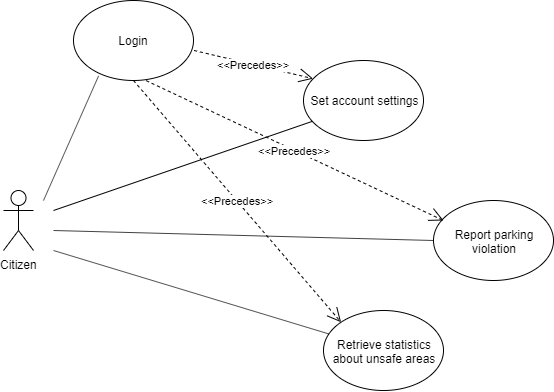
\includegraphics[scale=0.5]{img/Use_case_Citizen.png}
    \caption{Citizen Use Case Diagram}
\end{figure}
\clearpage
\begin{figure}[h!]
    \centering
    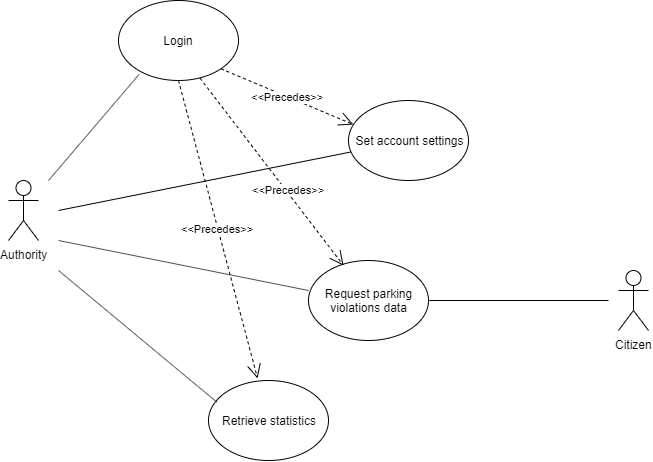
\includegraphics[scale=0.5]{img/Use_case_Authority.png}
    \caption{Authority Use Case Diagram}
\end{figure}

\subsubsection{Scenarios}
\begin{itemize}
    \item \textbf{Scenario 1}:
    Luca is walking towards work when outside, in the street of his , he sees that many cars are parked badly. 
    Some of these are parked near the strips, obstructing the view of the pedestrian who must cross the strips. 
    Luca tired of the situation that endangers him and many other citizens decides to report the incident to the police. 
    With his smartphone he opens the SafeStreets application and after logging in, click on the report button to report the fact. 
    Following the instructions of the luca application the necessary photo is taken, the plate is correctly recognized and 
    Luca then confirms the various data taken automatically. After the report Luca goes to statistics and discovers that it 
    is not the first time that the vehicle in question does not comply with the rules.

    \item \textbf{Scenario 2}:
    Luca is a disabled boy, he is perfectly able to drive the car but it is difficult for him to walk for long stretches. 
    The area in which he works is very busy and it is really difficult to find parking nearby but fortunately there are parking 
    spaces reserved for disabled people near the entrance of the building. One morning he finds the place occupied and looking 
    better note that the machine does not have the certificate necessary to be able to park in the places reserved for the disabled. 
    Thanks to Safestreet after logging in as a citizen, you can report this violation directly to the authorities by clicking on the report. 
    Following the instructions take the necessary photos directly from the application that retrieves information such as location and a 
    timestamp with date and time. The application tries to recognize the plaque from the photos and shows the result to Luca, who after 
    confirming the correctness can confirm and officially send the violation.

    \item \textbf{Scenario 3}:
    Il comando della municipale del comune di milano vuole ottimizzare i pattugliamenti, mirando alle zone più problematiche della città. 
    Questa sorveglianza mirata è fondamentale e porterebbe notevoli vantaggi tra cui: una potenziale riduzione di violazioni in queste aree 
    e riduzione di pattugliamenti inutili in aree con minor numero di violazioni. Fortunatamente, avendo aderito all'iniziativa di SafeStreet, 
    grazie al contributo dei cittadini possono utilizzare l'applicazione per ricevere queste statistiche direttamente da smartphone. Dopo essersi 
    registrati come autorità ed effettuato il login possono accedere alle statistiche visualizzando quindi le aree con più violazioni e i veicoli 
    di chi ha ricevuto più segnalazioni.

    \item \textbf{Scenario 4}:
    Andrea è un giovane vigile del comune di Milano. Ama mettere molta passione nel suo lavoro e per farlo si informa spesso verso le nuove tecnologie. 
    Dopo aver scaricato SafeStreet ed essersi registrato come Autorità si interessa subito alla funzione per generare multe grazie ai report fatti 
    dagli utenti. Dopo aver effettuato una richiesta viene visualizzata la schermata di riconoscimento in cui vengono mostrate le varie segnalazioni 
    una per volta. Andrea può comodamente valutare, osservando la foto, se effettivamente si tratta di una violazione e in caso affermativo andrea ha 
    tutti i dati necessari per poter generare una multa.
\end{itemize}

\subsubsection{Use Cases}
\clearpage
\begin{table}
    \begin{center}
    \centering
\begin{tabular}{ | l | l |}
\hline
\textbf{ID} & UC1 \\
\hline
\textbf{Description} & A \textit{Guest} creates a Citizen account \\
\hline
\textbf{Actors} & \textit{Guest} \\
\hline
\textbf{Precondition} & \textit{Guest}'s smartphone satisfies hardware limitations \\
             & \textit{Guest} has downloaded the app from the store \\
             & \textit{Guest} has not an account\\ 
\hline
\textbf{Flow of events} & 1. \textit{Guest} opens the app \\
                        & 2. \textit{Guest} clicks the registration button \\
                        & 3. \textit{System} asks which type of account he wants to create \\
                        & 4. \textit{Guest} selects Citizen account \\
                        & 5. \textit{System} shows the form \\
                        & 6. \textit{Guest} fills the form with his personal data plus mail and password \\
                        & 7. \textit{System} checks the validity of the data inserted \\
                        & 8. \textit{System} sends confirmation email \\
                        & 9. \textit{Guest} receives the email and clicks the URL to complete the registration \\  
\hline
\textbf{Postconditions} & \textit{System} has stored a new Citizen account  \\
                        & \textit{Guest} can login as Citizen \\
\hline
\textbf{Exceptions} & \textit{Guest} inserts an email that has been used by another account \\
                    & \textit{Guest} inserts a FC that has been inserted by another account \\
                    & In these case \textit{System} shows user an error message and the flow of events  \\
                    & restart from point 5 \\  
\hline
\end{tabular}
\caption{\textit{Guest} creates a Citizen account}
\end{center}
\end{table}


\clearpage
\begin{table}
    \begin{center}
    \centering
\begin{tabular}{ | l | l |}
\hline
\textbf{ID} & UC2 \\
\hline
\textbf{Description} & A \textit{Guest} creates a Authority account \\
\hline
\textbf{Actors} & \textit{Guest} \\
\hline
\textbf{Precondition} & \textit{Authority}'s smartphone satisfies hardware limitations \\
             & \textit{Guest} has downloaded the app from the store \\
             & \textit{Guest} has not an account\\ 
\hline
\textbf{Flow of events} & 1. \textit{Guest} opens the app \\
                        & 2. \textit{Guest} clicks the registration button \\
                        & 3. \textit{System} asks which type of account he wants to create \\
                        & 4. \textit{Guest} selects Authority account \\
                        & 5. \textit{System} shows the form \\
                        & 6. \textit{Guest} fills the form with his personal data plus P.IVA mail and password \\
                        & 7. \textit{System} checks the validity of the data inserted \\
                        & 8. \textit{System} sends confirmation email \\
                        & 9. \textit{Guest} receives the email and clicks the URL to complete the registration \\  
\hline
\textbf{Postconditions} & \textit{System} has stored a new Authority account  \\
                        & \textit{Guest} can login as Authority \\
\hline
\textbf{Exceptions} & \textit{Guest} inserts an email that has been used by another account \\
                    & \textit{Guest} inserts a P.IVA that has been inserted by another account \\
                    & In these case \textit{System} shows user an error message and the flow of events  \\
                    & restart from point 5 \\  
\hline
\end{tabular}
\caption{\textit{Guest} creates a Authority account}
\end{center}
\end{table}

\clearpage
\begin{table}
    \begin{center}
    \centering
\begin{tabular}{ | l | l |}
\hline
\textbf{ID} & UC3 \\
\hline
\textbf{Description} & A \textit{Citizen} logs in  \\
\hline
\textbf{Actors} & \textit{Citizen} \\
\hline
\textbf{Precondition} & \textit{Citizen} has already created the Citizen account \\
\hline
\textbf{Flow of events} & 1. \textit{Citizen} opens the app \\
                        & 2. \textit{Citizen} clicks the login button  \\
                        & 3. \textit{System} shows the form \\
                        & 4. \textit{Citizen} inputs his credentials  \\
                        & 5. \textit{System} checks the validity of the data inserted \\
\hline
\textbf{Postconditions} & \textit{Citizen} can use properly the app   \\
\hline
\textbf{Exceptions} & \textit{Citizen} inserts wrong credentials \\
                    & In this case \textit{System} shows user an error message and the flow of events  \\
                    & restart from point 3\\  
\hline
\end{tabular}
\caption{\textit{Citizen} login}
\end{center}
\end{table}

\clearpage
\begin{table}
    \begin{center}
    \centering
\begin{tabular}{ | l | l |}
\hline
\textbf{ID} & UC4 \\
\hline
\textbf{Description} & A \textit{Authority} logs in  \\
\hline
\textbf{Actors} & \textit{Authority} \\
\hline
\textbf{Precondition} & \textit{Authority} has already created the Authority account \\
\hline
\textbf{Flow of events} & 1. \textit{Authority} opens the app \\
                        & 2. \textit{Authority} clicks the login button  \\
                        & 3. \textit{Authority} clicks the login button for Authority \\
                        & 4. \textit{System} shows the form \\
                        & 5. \textit{Authority} inputs his credentials  \\
                        & 6. \textit{System} checks the validity of the data inserted \\
\hline
\textbf{Postconditions} & \textit{Authority} can use properly the app   \\
\hline
\textbf{Exceptions} & \textit{Authority} inserts wrong credentials \\
                    & In this case \textit{System} shows user an error message and the flow of events  \\
                    & restart from point 4\\  
\hline
\end{tabular}
\caption{\textit{Authority} login}
\end{center}
\end{table}

\clearpage
\begin{table}
    \begin{center}
    \centering
\begin{tabular}{ | l | l |}
\hline
\textbf{ID} & UC5 \\
\hline
\textbf{Description} & A \textit{Citizen} reports a parking violation  \\
\hline
\textbf{Actors} & \textit{Citizen} \\
\hline
\textbf{Precondition} & \textit{Citizen} has already logged in \\
\hline
\textbf{Flow of events} & 1. \textit{Citizen} clicks the report button \\
                        & 2. \textit{System} opens the photocamera \\
                        & 3. \textit{Citizen} takes a picture  \\
                        & 4. \textit{System} shows the summary \\
                        & 5. \textit{Citizen} inputs the type of violation \\
                        & 6. \textit{Citizen} clicks the send button \\
\hline
\textbf{Postconditions} & \textit{System}'s DB stores the violation  \\
\hline
\textbf{Exceptions} & \textit{Citizen} takes a bad picture \\
                    & In this case \textit{System} discards the picture and the flow of events  \\
                    & restart from point 3\\  
\hline
\end{tabular}
\caption{\textit{Citizen} reports a parking violation}
\end{center}
\end{table}

\clearpage
\begin{table}
    \begin{center}
    \centering
\begin{tabular}{ | l | l |}
\hline
\textbf{ID} & UC6 \\
\hline
\textbf{Description} & A \textit{Authority} retrieves a legitimate parking violation  \\
\hline
\textbf{Actors} & \textit{Authority} \\
\hline
\textbf{Precondition} & \textit{Authority} has already logged in \\
\hline
\textbf{Flow of events} & 1. \textit{Authority} clicks the retrieve button \\
                        & 2. \textit{System} shows summary of a parking violation \\
                        & 3. \textit{Authority} checks that it is a real parking violations  \\
                        & 4. \textit{Authority} clicks the ok button  \\
\hline
\textbf{Postconditions} &  \textit{Authority} generates a traffic and \textit{System} uploads \\ 
                        & statistics \\
\hline
\textbf{Exceptions} & \\ 
\hline
\end{tabular}
\caption{Legitimate parking violation retrieved by \textit{Authority} }
\end{center}
\end{table}

\clearpage
\begin{table}
    \begin{center}
    \centering
\begin{tabular}{ | l | l |}
\hline
\textbf{ID} & UC7 \\
\hline
\textbf{Description} & A \textit{Authority} retrieves a  wrong parking violation  \\
\hline
\textbf{Actors} & \textit{Authority} \\
\hline
\textbf{Precondition} & \textit{Authority} has already logged in \\
\hline
\textbf{Flow of events} & 1. \textit{Authority} clicks the retrieve button \\
                        & 2. \textit{System} shows summary of a parking violation \\
                        & 3. \textit{Authority} checks that it is not a real parking violations \\
                        & 4. \textit{Authority} clicks the discard button  \\
\hline
\textbf{Postconditions} & \textit{Authority} discards the picture and \textit{System} uploads   \\
                        &  statistics \\
\hline
\textbf{Exceptions} & \\ 
\hline
\end{tabular}
\caption{Wrong parking violation retrieved by \textit{Authority} }
\end{center}
\end{table}

\clearpage
\begin{table}
    \begin{center}
    \centering
\begin{tabular}{ | l | l |}
\hline
\textbf{ID} & UC8 \\
\hline
\textbf{Description} & A \textit{User} retrieves statistics  \\
\hline
\textbf{Actors} & \textit{Authority}, \textit{Citizen} \\
\hline
\textbf{Precondition} & \textit{User} has already logged in \\
\hline
\textbf{Flow of events} & 1. \textit{User} clicks the retrieve statistics button \\
                        & 2. \textit{System} shows summary of statistics \\
\hline
\textbf{Postconditions} & \textit{User} increases his knowledge about parking violations of his city  \\\
\hline
\textbf{Exceptions} & \\ 
\hline
\end{tabular}
\caption{statistics retrieved by \textit{User} }
\end{center}
\end{table}


\subsubsection{Sequence Diagrams}

\subsubsection{Goal Mapping on Requirements}

\subsection{Performance Requirements}
In this section we discuss requirements for what regards performance. The System must be able to support up to
1 million of registered users. This limitation is not posed by the front-end of the System, but rather by the 
back-end part, specifically the DB. For the same reasons it must be able to handle up to 1 million of parking violations 
sent by the \textit{Citizen}. In order to avoid any kind of saturation, every parking violation that has not been taken into account
 by any \textit{Authority} for 30 days, must be automatically discarded. This operation does not update the information about
 statistics.
 \\Requests about statistics shall be processed in less than 5 seconds. Requests about parking violations, instead, shall be processed 
 in less than 1 second.     

\subsection{Design Constraints}
\subsubsection{Standards compliance}
The S2B  will use certain measures as:
\begin{itemize}
    \item Standard longitude and latitude measures for the position
\end{itemize}
For what concerns the privacy, the S2B is subject to GDPR, a regulation in EU law on data protection 
and privacy for all individual citizens of UE  

\subsubsection{Hardware limitations}
In order to work properly the application must rely on hardwares that have certain requirements 
such as:
\begin{itemize}
    \item GPS
    \item internet connection (4G/3G/2G)
    \item Photocamera with a minimum precision of 5Mp 
\end{itemize}   

\subsection{Software System Attributes}
\subsubsection{Reliability}
The system must be able to run continuously without any interruptions. In order to do that, it must be ensured 
that the system is fault tolerant. To prevent downtime, one of the main goals of architecture design must be 
ensuring graceful degradation of the System
\subsubsection{Availability}
SafeStreets does not present any critical functions so 99\% availability with 3.65 days/year
as downtime shoud be good.  
\subsubsection{Security}
Security is a key aspect of SafeStreets because it is very important that the informations are never altered.
The S2B must:
\begin{enumerate}
 \item use HTTPS to safely communicate with the Server and DBMS    
 \item Hash the passwords so that they are not stored in clear in the DB
 \item Encrypt sensitive data before storing it
 \item digital sign the parking violation sent by Citizen and then hash it  
\end{enumerate} 
\subsubsection{Maintainability}
In order to achieve maintainability some good practices must be followed to reduce coupling and avoid code duplication 
\subsubsection{Portability}
S2B, as it stated previously, will work both in Andorid and iOS and this ensures itself portability. For 
the back-end part, it should be OS independent



%%%%%%%%%% !CHAPTER 3 %%%%%%%%%%


\section{Formal Analysis with Alloy}

\section{Efforts}


\end{document}